\begin{figure}[t]

    \begin{subfigure}[t]{0.3\textwidth}
        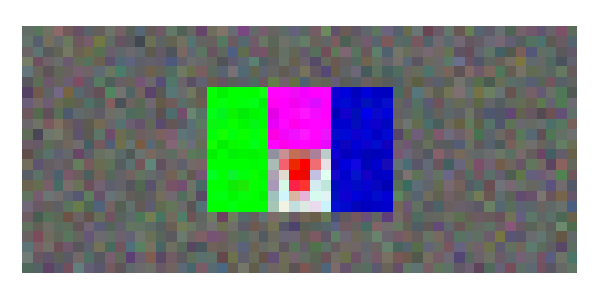
\includegraphics[width=\textwidth]{figures/OSC/TD1.pdf}
        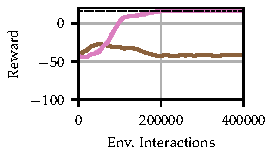
\includegraphics[width=\textwidth]{figures/OSC/cr_osc_6/OSC_TD1_lam05_reward_TigerDoor_True_v1_cr_osc_6_q0_2021_06_07__23_18_14_.pdf}
        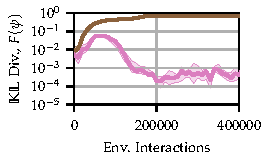
\includegraphics[width=\textwidth]{figures/OSC/cr_osc_6/OSC_TD1_lam05_divergence_TigerDoor_True_v1_cr_osc_6_q0_2021_06_07__23_18_14_.pdf}
        \caption{Tiger Door 1.}
        \label{supp:fig:grid:OSC:td1}
    \end{subfigure}%
    %
    \hfill%
    %
    \begin{subfigure}[t]{0.3\textwidth}
        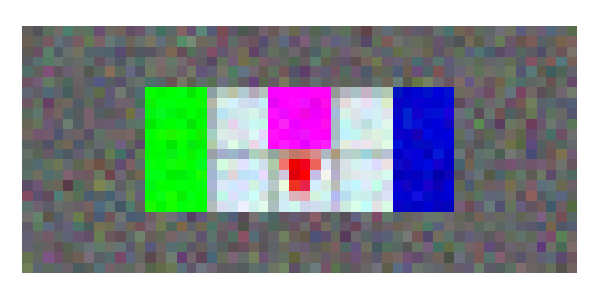
\includegraphics[width=\textwidth]{figures/OSC/TD2.pdf}
        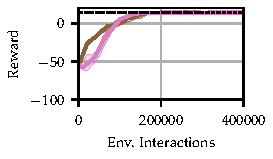
\includegraphics[width=\textwidth]{figures/OSC/cr_osc_6/OSC_TD2_lam05_reward_TigerDoor_True_v2_cr_osc_6_q0_2021_06_07__18_05_38_.pdf}
        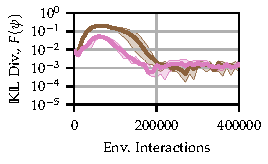
\includegraphics[width=\textwidth]{figures/OSC/cr_osc_6/OSC_TD2_lam05_divergence_TigerDoor_True_v2_cr_osc_6_q0_2021_06_07__18_05_38_.pdf}
        \caption{Tiger Door 2.}
        \label{supp:fig:grid:OSC:td2}
    \end{subfigure}%
    %
    \hfill%
    %
    \begin{subfigure}[t]{0.3\textwidth}
        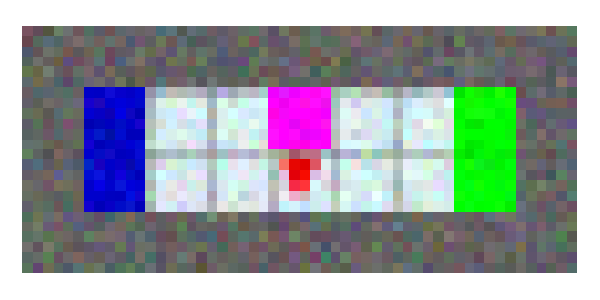
\includegraphics[width=\textwidth]{figures/OSC/TD3.pdf}
        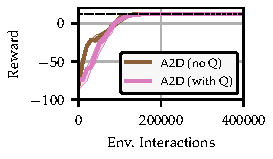
\includegraphics[width=\textwidth]{figures/OSC/cr_osc_6/OSC_TD3_lam05_reward_TigerDoor_True_v3_cr_osc_6_q0_2021_06_07__18_05_38_.pdf}
        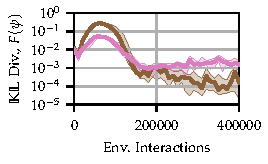
\includegraphics[width=\textwidth]{figures/OSC/cr_osc_6/OSC_TD3_lam05_divergence_TigerDoor_True_v3_cr_osc_6_q0_2021_06_07__18_05_38_.pdf}
        \caption{Tiger Door 3.}
        \label{supp:fig:grid:OSC:td3}
    \end{subfigure}%

    \caption{Results investigating requirement of directly estimating the Q function, as initially introduced in Section \ref{sec:algorithm} and discussed further in Section \ref{supp:sub:sub:q}.  Median and quartiles across $20$ random seeds are shown.  The Q function is learned targeting the expected discounted sum of rewards ahead conditioned on a particular (belief) state-action pair.  A value function is also learned in this way, and is used in conjunction with the Q function to directly estimate the advantage in \eqref{equ:a2d:a2d_update}.  Hence the A2D gradient is computed without direct use of Monte Carlo rollouts.  When no Q function is being used, the advantage is computed using GAE (c.f. Equations \eqref{equ:a2d:a2d_update}-\eqref{equ:a2d:gae}), with $\lambda = 0.5$.  We instantly anneal $\beta = 0$.  { }%  
    %
    Figure \ref{supp:fig:grid:OSC:td1}: Training curves for Tiger Door 1~\citep{littman1995pomdp}.  As predicted by the discussion in Section \ref{supp:sub:sub:q}, A2D does not converge to the correct policy if a Q function is not simultaneously learned.  This deficiency is instrumented by the high $\mathbb{KL}$ divergence throughout training and a discrepancy between the expected reward of the expert and agent.  If a Q function is learned, the desired partially observed behavior is recovered.   { }%
    %
    Figure \ref{supp:fig:grid:OSC:td2} and \ref{supp:fig:grid:OSC:td3}: By separating the goal by at least one square means the desired behavior is recovered regardless of whether a Q function is used.  This is because the bias has been reduced through the use of GAE and the introduction of additional random variables.  { }%
    }
    \label{supp:fig:grid:OSC}
\end{figure}